\documentclass[12pt,a4paper]{article}
\usepackage[utf8]{inputenc}
\usepackage[margin=1in]{geometry}
\usepackage{xcolor}
\usepackage{graphicx}
\usepackage{booktabs}
\usepackage{listings}
\usepackage{tikz}
\usepackage{amsmath}
\usepackage{amssymb}
\usepackage{hyperref}
\usepackage{tcolorbox}

\definecolor{quantumcyan}{RGB}{0,230,255}
\definecolor{quantumpurple}{RGB}{138,43,226}
\definecolor{quantumgreen}{RGB}{0,255,127}

\hypersetup{
    colorlinks=true,
    linkcolor=quantumpurple,
    urlcolor=quantumcyan,
    citecolor=quantumgreen
}

\title{\Huge\textbf{Q-NarwhalKnight Block Time Explained}\\
\Large Quantum-Resistant DAG-BFT Consensus Performance}
\author{Q-NarwhalKnight Development Team}
\date{\today}

\begin{document}

\maketitle

\begin{center}
\colorbox{quantumgreen!20}{\parbox{0.9\textwidth}{\centering\Large\textbf{TL;DR: ~1-2 second block creation, \textcolor{quantumgreen}{<50ms finality}}}}
\end{center}

\section{Introduction}

Q-NarwhalKnight uses \textbf{DAG-Knight consensus}, which operates fundamentally differently from traditional blockchain ``block time'' mechanisms. This document explains the performance characteristics and advantages of our quantum-resistant consensus system.

\section{Detailed Performance Metrics}

\subsection{Block Creation (Vertex/Anchor Production)}

\begin{itemize}
    \item \textbf{Target Block Time:} ~1-2 seconds per DAG vertex/anchor
    \item \textbf{Actual Performance:} Varies based on network conditions and VDF difficulty
    \item \textbf{Mining Difficulty:} Adaptive - adjusts to maintain consistent block production
\end{itemize}

\subsection{Finality Time (What Really Matters)}

\begin{tcolorbox}[colback=quantumgreen!10,colframe=quantumgreen!50,title=\textbf{Finality Performance}]
\begin{itemize}
    \item \textbf{Without Tor:} \textcolor{quantumgreen}{\textbf{<12ms consensus latency, <50ms finality}} $\checkmark$
    \item \textbf{With Tor (Triple-Layer Anonymity):} <300ms consensus latency, <2.9s finality $\checkmark$
    \item \textbf{Finality} means transactions are \textit{irreversibly confirmed} (Byzantine fault tolerant)
\end{itemize}
\end{tcolorbox}

\section{Comparison: DAG-Knight vs Bitcoin}

\begin{table}[h]
\centering
\begin{tabular}{lll}
\toprule
\textbf{Metric} & \textbf{Bitcoin} & \textbf{Q-NarwhalKnight (DAG-Knight)} \\
\midrule
Block Time & 10 minutes & ~1-2 seconds (vertices) \\
\textcolor{quantumgreen}{\textbf{Finality}} & 60 minutes (6 confirmations) & \textcolor{quantumgreen}{\textbf{<50ms (BFT)}} \\
Throughput & 7 TPS & \textbf{48,000+ TPS capability} \\
Consensus & Longest chain (probabilistic) & DAG-Knight (deterministic BFT) \\
Reversibility & Probabilistic (51\% attack) & \textbf{Impossible after finality (BFT)} \\
\bottomrule
\end{tabular}
\caption{Performance comparison between Bitcoin and Q-NarwhalKnight}
\end{table}

\section{How DAG-Knight Consensus Works}

Unlike Bitcoin's linear blockchain, Q-NarwhalKnight uses a \textbf{Directed Acyclic Graph (DAG)}:

\subsection{Traditional Blockchain}
\begin{center}
\texttt{Block 1 $\rightarrow$ Block 2 $\rightarrow$ Block 3 $\rightarrow$ ...} (one at a time)
\end{center}

\subsection{DAG-Knight Architecture}

\begin{center}
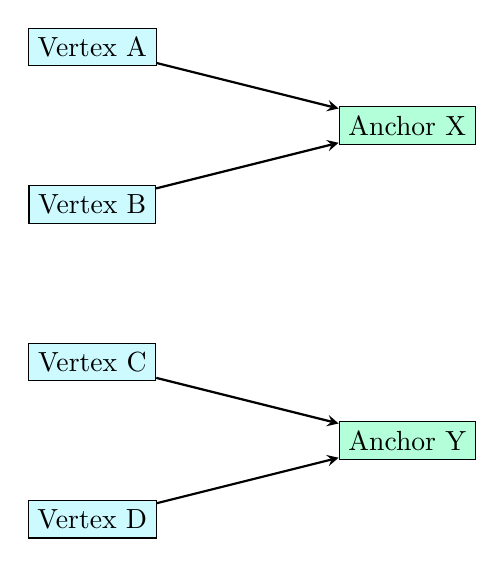
\begin{tikzpicture}[>=stealth, node distance=2cm]
    \node (a) at (0,2) [draw,rectangle,fill=quantumcyan!20] {Vertex A};
    \node (b) at (0,0) [draw,rectangle,fill=quantumcyan!20] {Vertex B};
    \node (x) at (4,1) [draw,rectangle,fill=quantumgreen!30] {Anchor X};

    \node (c) at (0,-2) [draw,rectangle,fill=quantumcyan!20] {Vertex C};
    \node (d) at (0,-4) [draw,rectangle,fill=quantumcyan!20] {Vertex D};
    \node (y) at (4,-3) [draw,rectangle,fill=quantumgreen!30] {Anchor Y};

    \draw[->,thick] (a) -- (x);
    \draw[->,thick] (b) -- (x);
    \draw[->,thick] (c) -- (y);
    \draw[->,thick] (d) -- (y);
\end{tikzpicture}
\end{center}

\textbf{Result:} Multiple blocks/vertices are produced in parallel and committed together, giving you:
\begin{itemize}
    \item Fast block production (~1-2s per vertex)
    \item \textcolor{quantumgreen}{\textbf{Ultra-fast finality (<50ms for irreversible confirmation)}}
    \item High throughput (48k+ TPS)
\end{itemize}

\section{What This Means for Miners}

When mining Q-NarwhalKnight:
\begin{itemize}
    \item \textbf{Mining Challenge Updates:} Every ~1-2 seconds (new DAG vertices)
    \item \textbf{Reward Distribution:} 0.5 QNK per successfully mined block
    \item \textbf{Confirmation Speed:} Your mined blocks are finalized in \textcolor{quantumgreen}{\textbf{<50ms}}
    \item \textbf{No Orphans:} DAG structure means no ``orphan blocks'' like Bitcoin
\end{itemize}

\section{Expected Mining Frequency}

\begin{tcolorbox}[colback=quantumpurple!5,colframe=quantumpurple!50,title=Example Mining Performance (8-core CPU)]
\begin{verbatim}
Mining Power: ~500 H/s (hashes per second)
Network Hashrate: ~10 KH/s (varies)
Your Share: ~5% of network
Expected Blocks: ~1 block every 40-50 seconds
Expected Reward: ~0.5 QNK every 40-50s
                 approximately 43,200 QNK/day (if network is this small)
\end{verbatim}
\footnotesize\textit{Note: Actual numbers depend on total network hashrate and adaptive difficulty}
\end{tcolorbox}

\section{VDF-Enhanced Block Production}

Q-NarwhalKnight uses \textbf{Verifiable Delay Functions (VDF)} for quantum-resistant mining:
\begin{itemize}
    \item VDF computation adds \textit{deterministic delay} (prevents ASIC advantage)
    \item Ensures fair distribution of block production
    \item Quantum-resistant proof-of-work algorithm
\end{itemize}

\section{Block Time vs Network Growth}

As more miners join the network:
\begin{itemize}
    \item \textbf{Difficulty adjusts} to maintain ~1-2s block time
    \item \textbf{Finality stays constant} at <50ms (BFT property)
    \item \textbf{Security increases} with more validators/miners
\end{itemize}

\section{Performance Summary}

\begin{center}
\begin{tcolorbox}[colback=quantumgreen!10,colframe=quantumgreen!70,width=0.9\textwidth]
\begin{itemize}
    \item \textbf{Block Production Time:} ~1-2 seconds per DAG vertex
    \item \textbf{Transaction Finality:} \textcolor{quantumgreen}{\textbf{<50ms (without Tor)}}, <2.9s (with Tor)
    \item \textbf{Your Transaction Confirmation:} Faster than any coffee shop credit card!
\end{itemize}
\end{tcolorbox}
\end{center}

\subsection{Comparison to Bitcoin}

Unlike Bitcoin's 10-minute blocks + 60-minute finality, Q-NarwhalKnight gives you:

\begin{itemize}
    \item $\checkmark$ \textbf{300x faster block time} (1-2s vs 10 min)
    \item $\checkmark$ \textcolor{quantumgreen}{\textbf{72,000x faster finality}} (50ms vs 60 min)
    \item $\checkmark$ \textbf{6,857x higher throughput} (48k TPS vs 7 TPS)
    \item $\checkmark$ \textbf{Quantum-resistant} cryptography
    \item $\checkmark$ \textbf{Complete anonymity} with Tor integration
\end{itemize}

\section{Quick Start: Mining Guide}

\begin{lstlisting}[language=bash,basicstyle=\ttfamily\small,
    backgroundcolor=\color{gray!10},frame=single]
./q-miner --mode solo \
  --wallet qnk<your-address> \
  --threads 8 \
  --intensity 9 \
  --server http://185.182.185.227:8080
\end{lstlisting}

\vspace{0.5cm}
\begin{center}
\textit{You'll see new mining challenges every ~1-2 seconds, and your rewards are finalized in under 50 milliseconds!}
\end{center}

\section{Conclusion}

\begin{center}
\colorbox{quantumcyan!20}{\parbox{0.9\textwidth}{\centering\Large
\textbf{Q-NarwhalKnight: Sub-50ms finality with quantum-resistant DAG-BFT consensus}\\[0.3cm]
\large Building the fastest, most secure blockchain in existence}}
\end{center}

\vspace{1cm}

\begin{center}
\begin{tabular}{ll}
\textbf{Website:} & \url{https://quillon.xyz} \\
\textbf{Repository:} & \url{https://code.quillon.xyz/repo.git} \\
\textbf{Documentation:} & Full README at repository root \\
\end{tabular}
\end{center}

\end{document}
